
\subsection{Execution graph}\label{abstrCntrFlow}
We denote by $\Gamma  = ( \Omega, \ll)$ the execution graph of a
bytecode $\Pi$ where the set of nodes $\Omega$ is the set of
blocks. The set of edges $\ll$ defines the execution relation
between blocks.Using standard terminology \cite{ARUCom1986}, a
basic block is a code segment that has no unconditional jump or
conditional branch statements except for possibly the last
statement, and none of its statements, except possibly the first,
is a target of any jump or branch statement. The formal definition of block follows
below.

We denote a block that starts at instruction $\tt{i_{j}}$
respectively by \blockm{j}. Let's have the bytecode $\Pi$ and the
set of its blocks  be $\wp$. The edges ( $\ll \ \subseteq \wp \ \times \ \wp $ ) define the order of block execution.

\begin{defn}[Execution relation between blocks]\label{execRel}
\begin{tabbing}
\\Let \=  have \= the block \blockm{j} such that  it ends with instruction $\tt{i_{k}}$ and \\
it is not a return instruction\\
\>  if $\tt{i_{k}}$ = \texttt{if\_cond n} then   \blockm{j} $\ll$ \blockm{n} and \blockm{j}  $\ll $ \blockm{k+1}  \\
\>  if $\tt{i_{k}}$ = \texttt{goto n} then \blockm{j} $\ll$ \blockm{n} \\
\>  if $\tt{i_{k}}$ = \texttt{jsr n} then \blockm{j} $\ll$ \blockm{n} \\
\>  if $\tt{i_{k}}$ = \texttt{athrow} then \blockm{j} $\ll$ \blockm{n} for all \texttt{n}, such that \blockm{n} is the first\\
\> \> block of an exception handler that protects $\tt{i_{k}}$ \\
\>  if  $\tt{i_{k}}$ = \texttt{ret n} then  \blockm{j} $\ll$ \blockm{s}\\
\> \> for all s that are indexes of instruction following \\
\> \> a \texttt{jsr} to the subroutine that ends with $\tt{i_{k}}$ instruction\\
\>  else \blockm{j} $ \ll  $ \blockm{k+1}
\end{tabbing}
\end{defn}
%We say that $\tt{instr_{i}} $ is a precedent of $\tt{instr_{j}}$  and that  $\tt{instr_{j}}$ is next to  $\tt{instr_{i}}$ if $\tt{instr_{i}} \ll \tt{instr_{j}} $ , the same for blocks that are in the same relation.
We say that there exists a path between \blockm{i} and \blockm{j} and we note it with  \pathm{i}{j}, if there exists blocks \blockm{s_{1}}... \blockm{s_{n}} such that \blockm{i}$\ll$ \blockm{s_{1}}$\ll$ \blockm{s_{2}}... \blockm{s_{n}}$\ll$ \blockm{j}
\begin{defn}[Loop Definition]
\label{defLoop}
Let's have a well formed program $\Pi$. We say that \blockm{s} is the start block of loop $l$ in $\Pi$ and \blockm{e} is the end block of $l$ if:
\begin{itemize}
\item there exists a path in the execution graph starting at the entry block \blockm{entry} (i.e. the one that starts with the entry instruction) of $\Pi$ and that passes first through \blockm{s} and later through \blockm{e}, i.e.\blockm{entry} $\ll^{*}$ \blockm{s} $\ll^{*}$ \blockm{e}
\item \blockm{e} $\ll$ \blockm{s}
\end{itemize}
\end{defn}

%Loops are represented as cycles in the execution graph. Every loop has a unique name $ \tt{ loop_{i}}$  Every loop $\tt{loop_{i}}$ in a well formed program is defined uniquely by two  instructions - the first instruction of the loop  $\tt{loop^{i}_{start}}$  and the last instruction of the loop $\tt{loop^{i}_{end}}$  and by definition they are in relation $\ll$.

%Relation $\ll$ defines also an execution relation between blocks $\ll$ (we use the same name for the instruction and block execution relation)
%\begin{defn}{Execution relation between blocks}
%\label{execRel}
%Let $\tt{b^{1}}$ and $\tt{b^{2}}$ are blocks. $\tt{b^{1}} \ll \tt{b^{2}} \iff \tt{b^{1}_{end}} \ll \tt{b^{2}_{start}}$.
%\end{defn}


\subsection{Acyclic Execution Graph} \label{graph}
We consider the acyclic graph $\Gamma^1 = ( \Omega, \ll^1)$ obtained from the execution graph $\Gamma  = ( \Omega, \ll)$ of a well formed bytecode $ \Pi $. The set of nodes $\Omega$ is the set of  blocks in the program and the relation  $\ll^1 $ is a subset of the  execution relation $\ll$.
\begin{defn}[Acyclic Execution relation]
\label{acyclicExRel}
Let's have the well formed bytecode program $\Pi$ and let have in $\Pi$ the two blocks  \blockm{i} and   \blockm{j}. We say that \blockm{i} $\ll^{1}$ \blockm{j} iff
\begin{itemize}
\item \blockm{i} $\ll$ \blockm{j}
\item and block \blockm{i} and block \blockm{j} are not the end and the start blocks respectively of the same loop, see loop definition~\ref{defLoop}.
\end{itemize}
\end{defn}

%Naturally $\ll^1$ defines a relation between blocks for which we use the same notation $\ll^1$ .
Both the cyclic and acyclic graphs of the bytecode of method \texttt{half} at Fig.~\ref{halfBC} is at Fig. ~\ref{blockBC}. Blocks are represented by boxes. Black arrows stand for relation $\ll^1$. Dashed arrows represent relation $\ll$.

\begin{figure}[p]
\begin{center}
\begin{tabular}{rl}
 0 & iconst\_0\\ 
 1 & istore\_2\\
 2 & iload\_1\\
 3 & istore\_3\\%[-2mm]
 4 & goto 13 (+9)\\%[-2mm]
 7 & iinc 2 by 1\\%[-2mm]
10 & iinc 1 by 254\\%[-2mm]
13 & iload\_1\\%[-2mm]
14 & iconst\_1\\%[-2mm]
15 & if\_icmpgt 7 (-8)\\%[-2mm]
18 & iload\_2\\%[-2mm]
19 & ireturn\\%[-2mm]
\end{tabular}
\end{center}
\caption{the bytecode of method \texttt{half}}
\label{halfBC}
\end{figure}

\begin{figure}[p]
\begin{center}
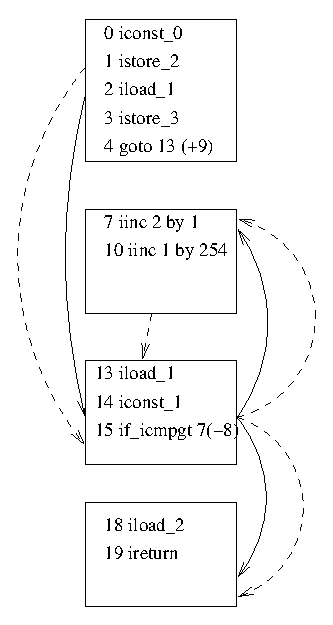
\epsfig{file=graph.eps}
\end{center}
\caption{bytecode blocks of bytecode at Figure ~\ref{halfBC}}
\label{blockBC}
\end{figure}

Now a path in $\Gamma^1$  is a list of blocks between which is established a relation $\ll^1$ and that starts at the entry point instruction and whose last block is a block that does not have next block.

